\documentclass[12pt]{exam}
\usepackage{amsmath}
\usepackage{amssymb}
\usepackage{graphicx}
\usepackage{enumitem}
\usepackage{amsfonts}
\usepackage{amssymb}
\usepackage{ifthen}
\usepackage{geometry}
\noprintanswers

\usepackage{tikz}
\usetikzlibrary{shapes,backgrounds}

\addtolength{\textheight}{3cm}
\addtolength{\topmargin}{-1cm}
\addtolength{\textwidth}{3cm}
\addtolength{\oddsidemargin}{-1.5cm}
\addtolength{\evensidemargin}{-1.5cm}
\setlength\parindent{0pt}

\newcommand {\DS} [1] {${\displaystyle #1}$}
\newcommand{\vv}{\vspace{.2cm}}

\newcommand{\R}{\mathbb{R}}
\newcommand{\C}{\mathbb{C}}
\newcommand{\Z}{\mathbb{Z}}
\newcommand{\N}{\mathbb{N}}

\pagestyle{empty}


%============================================
%user setting
%============================================

\graphicspath{ {./images/} }

%============================================
%137 COLOUR PALETTE
%============================================

\definecolor{137cp1}{RGB}{13, 33, 161}
\definecolor{137cp2}{RGB}{51, 161, 253}
\definecolor{137cp3}{RGB}{255, 67, 101}
\definecolor{137cp4}{RGB}{232, 144, 5}


%============================================
%HYPERLINKS
%============================================

\usepackage{hyperref}
\hypersetup{colorlinks}
\hypersetup{urlcolor=137cp3, linkcolor=137cp1}

%%%%%%%%%%%%%%%%%%%%%%%%%%%%%%%%%%%%%%%%%


\begin{document}

{\large
	\begin{center}
		{\bf MAT 137Y: Calculus with proofs}\\
		{\bf Assignment 2} \\
		{\bf Due on Thursday, October 15 by 11:59pm via Crowdmark}
	\end{center}
}

\vv

\begin{quotation}
{\bf Instructions:}
	\begin{itemize}
		\item	 You will need to submit your solutions electronically via Crowdmark.   \href{https://www.math.toronto.edu/~alfonso/137/PS/137_CM.html}{See MAT137 Crowdmark help page for instructions}.  Make sure you understand how to submit and that you try the system ahead of time.  If you leave it for the last minute and you run into technical problems, you will be late.  There are no extensions for any reason.
		\item You may submit individually or as a team of two students.  See the link above for more details.
		\item  You will need to submit your answer to each question separately.
		\item  This problem set is about the the definition and basic properties of limits (Unit 2 up to Video 2.13).
	\end{itemize}
\end{quotation}
\vv

\begin{enumerate}

\setcounter{enumi}{-1}

\item Read \href{https://www.math.toronto.edu/~alfonso/137/PS/137_2021_collaboration.pdf}{``Notes on collaboration"} on the course website.

	Write out the following sentence and sign below it, to certify that you have read it.
	
	\begin{quote}
		``I have read and understood the notes on collaboration for this course, as explained in the course website."
	\end{quote}

\vv

\newpage

\item \emph{Note:} Before you attempt this question, solve Q1 and Q3 on the practice problems for Unit 2.  Otherwise, you will find this question too hard.

  Sketch the graph of a function $h$ that satisfies all the following properties at once:
	\begin{enumerate}
		\item The domain of $h$ is $\R$.
		\item  \DS{\lim_{x \to 2} h(x) = 0} \; and \; \DS{\lim_{x \to 2} h(h(x)) = \infty}.
		\item  \DS{\lim_{x \to 4} h(x) = 0} \; and \; \DS{\lim_{x \to 4} h(h(x)) = - \infty}.
		\item \DS{\lim_{x \to 0} h(h(x))=3}.
		\item  \DS{\lim_{x \to -3^+} h(x) = 0} \; and \\
		   \DS{\lim_{x \to -3^+} h(h(x))} does not exist, is not $\infty$, and is not $-\infty$.
	\end{enumerate}
	To clarify, we want one single function $h$ that satisfies all the conditions in all the parts, all at once.  Make your graph tidy and unambiguous.  If necessary, add words to explain what is happening in the graph.  
\vv

\textbf{the picture of the function h is on the next page.}\\
Here is the definition of function $h$ that satisfies conditions a-e all at once.\\

\vv

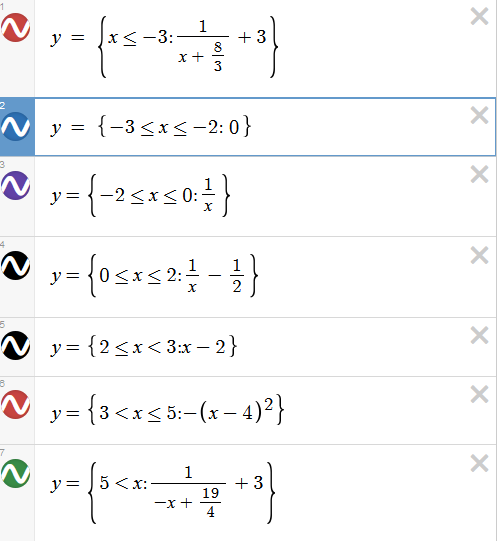
\includegraphics[scale = 0.8]{definition.png}\\

\newpage
Here is what the function looks like.
\vv

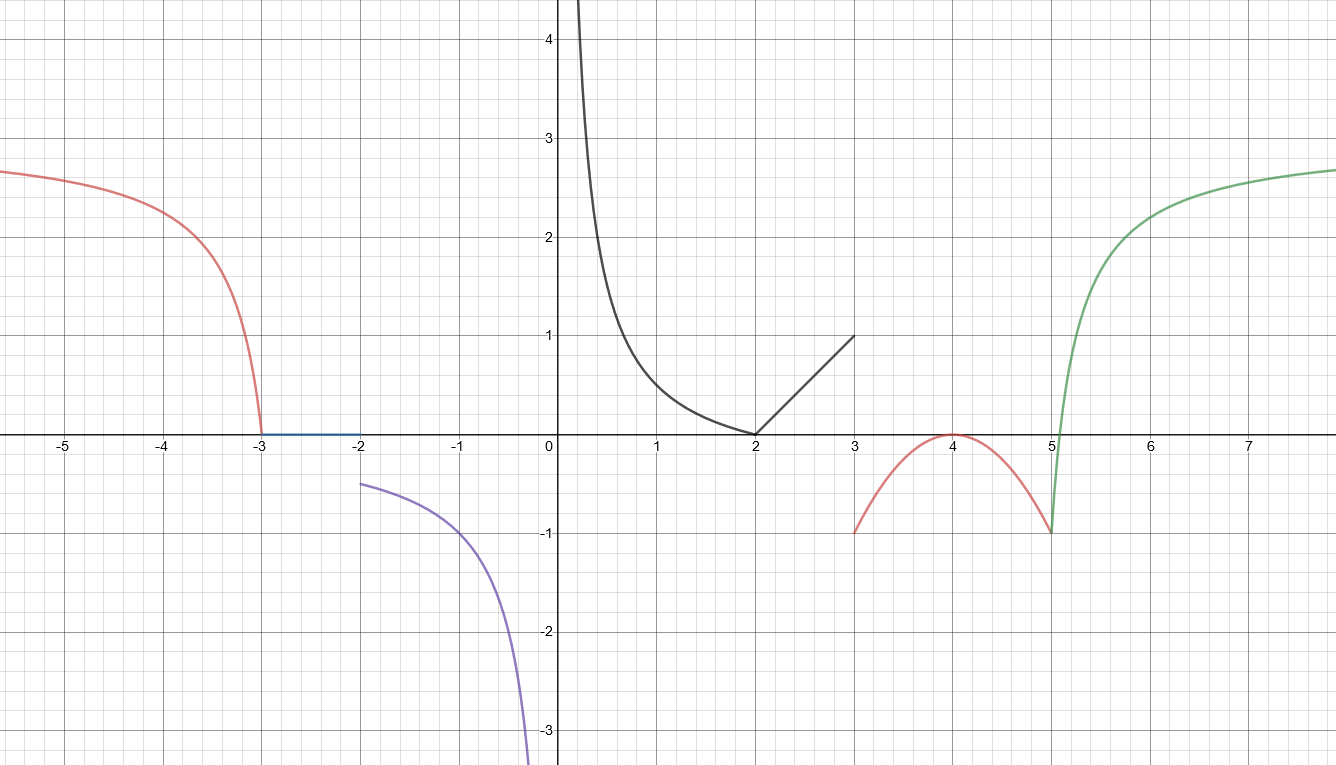
\includegraphics[scale = 0.5]{function graph.png}


\newpage

\item  Let \DS{a \in \R}.  Let $f$ and $g$ be two functions that are defined, at least, on an interval centered at $a$, except maybe at $a$.  
Assume that \DS{\lim_{x \to a} f(x)} does not exist, and that \DS{\lim_{x \to a} g(x)} does not exist.  Based only on this information, can you conclude whether \DS{\lim_{x \to a}\left[f(x) + g(x) \right]} exists or does not exist?  Prove it.

\vv  

\newpage


\item Prove that \DS{\lim_{x \to 2} x^3 = 8}.  Write a proof directly from the definition of limit, without using any of the limit laws or other theorems.

\vv

\newpage


\item  Let $f$ and $g$ be two functions with domain $\R$. Let \DS{h = f+ g}.  Prove that
	\begin{center}
	\begin{tabular}{ll}
			IF &
			\DS{\lim_{x \to \infty} f(x)  = \infty \quad \mbox{ and } \quad \lim_{x \to \infty} g(x) \mbox{ exists}},
			\\
			THEN \quad &
			\DS{\lim_{x \to \infty} h(x) = \infty}.
	\end{tabular}
	\end{center}
Write a proof directly from the definition of limit, without using any of the limit laws or other theorems.

\end{enumerate}
\end{document}


